\documentclass[aspectratio=169]{beamer}

% ---------- THEME & LOOK ----------
\usetheme{Madrid}
\usecolortheme{seahorse}
\usefonttheme{professionalfonts}
\setbeamertemplate{navigation symbols}{}
\setbeamercovered{transparent}
\setbeamertemplate{itemize items}[circle]
\setbeamertemplate{enumerate items}[default]
\setlength{\parskip}{0.25em}

% ---------- COLORS ----------
\usepackage{xcolor}
\definecolor{accent}{RGB}{0,92,184}
\definecolor{soft}{RGB}{233,244,255}
\setbeamercolor{structure}{fg=accent}
\setbeamercolor{title}{fg=white,bg=accent}
\setbeamercolor{frametitle}{fg=accent}
\setbeamercolor{block title}{bg=accent!10,fg=accent}
\setbeamercolor{block body}{bg=soft}

% ---------- PACKAGES ----------
\usepackage{booktabs}
\usepackage{amsmath, amssymb}
\usepackage{array}
\usepackage{hyperref}
\hypersetup{colorlinks=true,linkcolor=accent,urlcolor=accent}

% ---------- PLACEHOLDER BOX ----------
\newcommand{\placeholderbox}[2][0.82\linewidth]{%
  \begin{center}
    \fbox{\begin{minipage}[c][0.46\textheight][c]{#1}
      \centering \vspace{0.25em}
      \textbf{#2}\\[0.6em]
      \emph{Insert figure/diagram here later.}
    \end{minipage}}
  \end{center}
}

% ---------- TITLE ----------
\title{\textbf{Compensating Wage Differentials \vspace{.5cm}\\  }}
\subtitle{{\large ECON 300 - Labour Economics}}
\author{Muhebullah Karimzada}
\date{Winter 2026}

\begin{document}

% ============================================================
% TITLE
% ============================================================
\begin{frame}[plain]
  \titlepage
\end{frame}

% ============================================================
\section{Orientation}
% ============================================================

\begin{frame}{Learning Objectives}
\transfade
\begin{itemize}
  \item Explain how wages reflect job attributes such as \textbf{working conditions, safety risks, shift work, pensions, and health benefits}.
  \item Understand the meaning of \textbf{compensating wage differentials}: wage differences that compensate workers for undesirable job characteristics.
  \item Identify when market-determined workplace risk may be \textbf{efficient} and when market outcomes may fail.
  \item Evaluate how \textbf{safety regulation} affects workers, firms, and total welfare.
  \item Understand the principle of \textbf{``no free lunch''}: desirable job amenities are often accompanied by \textbf{lower wages}.
  \item Use wage premiums for risky jobs to infer the \textbf{value of a statistical life (VSL)}.
\end{itemize}
\end{frame}

\begin{frame}{Main Questions}
\transfade
\begin{itemize}
  \item What determines relative pay rates across jobs?
  \item Can equally skilled workers earn different wages in the neoclassical model?
  \item Why do some unpleasant or dangerous jobs pay more?
  \item Do safety regulations always improve worker welfare?
  \item Are workers fully compensated for risky or undesirable job attributes?
\end{itemize}
\end{frame}

\begin{frame}{Big Idea of the Chapter}
\transfade
\begin{block}{Core Insight}
Wages do not only pay for \textbf{skills and productivity}. They also reflect \textbf{job characteristics} such as risk, discomfort, flexibility, and fringe benefits.
\end{block}
\begin{itemize}
  \item Workers trade off \textbf{money wages} against \textbf{non-wage job characteristics}.
  \item Firms choose combinations of wages and job attributes that minimize cost or maximize profit.
  \item Market equilibrium emerges through \textbf{sorting}: different workers choose different jobs.
\end{itemize}
\end{frame}

% ============================================================
\section{Purposes of Wages and Wage Structures}
% ============================================================

\begin{frame}{Purposes of Wages and Wage Structures}
\transfade
\begin{block}{Definition: Wage Structure}
The \textbf{wage structure} is the hierarchy or grid of wages across jobs. It includes wage \textbf{premiums} linked to worker skills, job tasks, working conditions, and amenities.
\end{block}
\begin{itemize}
  \item \textbf{Wage -- productivity link:} In competitive settings, wages must reflect marginal productivity.
  \item \textbf{Compensation role:} Jobs with unpleasant or risky conditions often require higher wages.
  \item \textbf{Organizational role:} Wages also help with motivation, fairness, recruitment, and retention.
  \item \textbf{Example:} Miners or offshore workers often earn more than office workers partly because of risk and harsh conditions.
\end{itemize}
\end{frame}

\begin{frame}{Why Can Similar Workers Earn Different Wages?}
\transfade
\begin{itemize}
  \item Even equally skilled workers may earn different wages if jobs differ in:
  \begin{itemize}
    \item workplace safety,
    \item scheduling convenience,
    \item pensions and health insurance,
    \item location and commuting burden,
    \item employment stability.
  \end{itemize}
  \item These differences are called \textbf{compensating wage differentials}.
  \item Thus, wage inequality may reflect both \textbf{worker characteristics} and \textbf{job characteristics}.
\end{itemize}
\end{frame}

% ============================================================
\section{Theory of Compensating Wages}
% ============================================================

\begin{frame}{Smith's Compensating Differentials: What Gets Priced?}
\transfade
\begin{block}{Historical Insight}
Adam Smith argued that wage differences across occupations reflect the \textbf{advantages and disadvantages} attached to different jobs.
\end{block}
\begin{itemize}
  \item Agreeableness or disagreeableness of tasks
  \item Training cost and difficulty
  \item Job stability and probability of success
  \item Responsibility, trust, and authority
  \item \textbf{Safety and risk}
\end{itemize}
\end{frame}

\begin{frame}{Definition: Compensating Wage Differential}
\transfade
\begin{block}{Definition}
A \textbf{compensating wage differential} is the extra wage required to persuade workers to accept an undesirable job characteristic, or the wage reduction they accept for a desirable characteristic.
\end{block}
\begin{itemize}
  \item Dangerous jobs often require a \textbf{wage premium}.
  \item Pleasant or flexible jobs may pay \textbf{less} because workers value the amenity.
  \item Example: A safer office job may pay less than a riskier construction job for equally skilled workers.
\end{itemize}
\end{frame}

\begin{frame}{Isoprofit Schedules (Firms' Side)}
\transfade
\begin{block}{Definition: Isoprofit Curve}
An \textbf{isoprofit schedule} shows all combinations of \textbf{wage} and \textbf{safety} that yield the same profit for the firm.
\end{block}
\begin{itemize}
  \item Firms can compensate workers by paying higher wages or by providing safer conditions.
  \item Improving safety may require spending on equipment, training, or monitoring.
  \item Lower isoprofit curves correspond to \textbf{higher profits}.
  \item The slope reflects the firm's trade-off between safety spending and wage costs.
\end{itemize}
\end{frame}

\begin{frame}{Figure 8.1: Employer's Isoprofit Schedules and Offer Curve}
\centering
\vspace{3.5em}
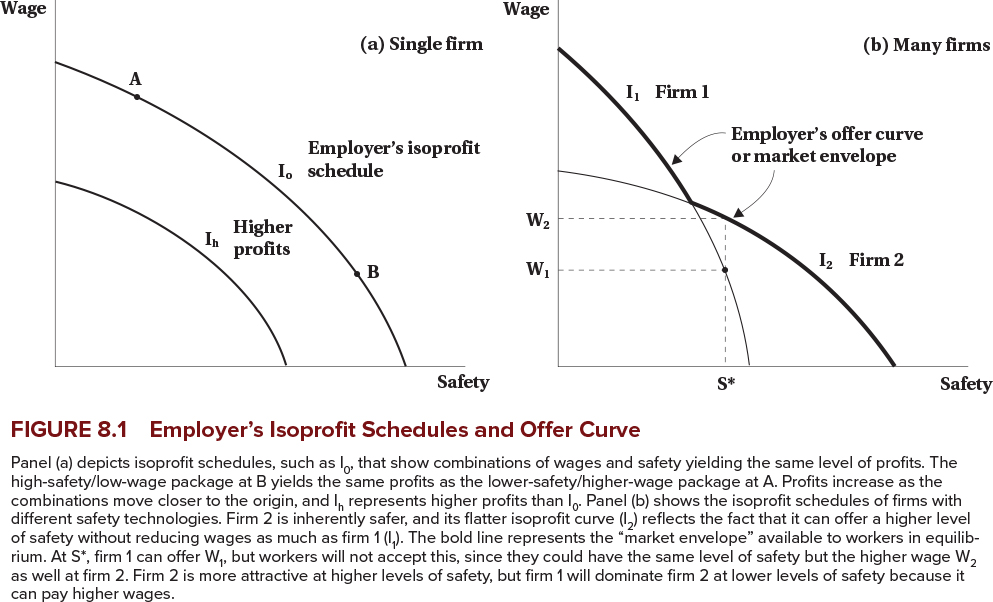
\includegraphics[width=0.99\linewidth]{ben54842_0801}
\end{frame}

\begin{frame}{Explaining Figure 8.1}
\transfade
\begin{itemize}
  \item Each isoprofit curve shows wage -- safety combinations that give the same profit.
  \item Curves farther from the origin generally imply \textbf{lower profits}.
  \item Tangency between isoprofit schedules and workers' preferences determines feasible offers.
  \item The \textbf{offer curve} traces the combinations of wage and safety that firms are willing to offer as worker preferences differ.
\end{itemize}
\end{frame}

\begin{frame}{Different Safety Technologies Across Firms}
\transfade
\begin{itemize}
  \item Firms differ in the \textbf{cost of providing safety}.
  \item Some firms can improve safety cheaply; others face high safety costs.
  \item Therefore, even for the same profit level, firms may have \textbf{different isoprofit curves}.
  \item Example: A modern factory may provide safety more cheaply than an old mine.
\end{itemize}
\end{frame}

\begin{frame}{Worker Preferences and Indifference Curves}
\transfade
\begin{block}{Definition: Indifference Curve}
An \textbf{indifference curve} shows combinations of \textbf{wage} and \textbf{safety} that give the worker the same utility.
\end{block}
\begin{itemize}
  \item Workers prefer:
  \begin{itemize}
    \item higher wages,
    \item safer jobs.
  \end{itemize}
  \item More risk-averse workers require larger wage premiums to accept danger.
  \item Thus, worker heterogeneity is central to compensating wage theory.
\end{itemize}
\end{frame}

\begin{frame}{Figure 8.2: Worker Indifference Curves}
\centering
\vspace{5em}
\includegraphics[width=0.9\linewidth]{ben54842_0802}
\end{frame}

\begin{frame}{Explaining Figure 8.2}
\transfade
\begin{itemize}
  \item Each indifference curve shows wage -- safety bundles that leave the worker equally well off.
  \item Higher indifference curves imply \textbf{higher utility}.
  \item A steep indifference curve means the worker values safety highly and requires a large wage increase to accept more risk.
  \item A flatter indifference curve means the worker is more willing to trade safety for wages.
\end{itemize}
\end{frame}

\begin{frame}{Equilibrium with One Firm and One Worker}
\transfade
\begin{itemize}
  \item The optimal wage -- safety bundle occurs at the \textbf{tangency} of:
  \begin{itemize}
    \item the firm's isoprofit curve, and
    \item the worker's indifference curve.
  \end{itemize}
  \item At tangency:
  \begin{itemize}
    \item the worker cannot be made better off without lowering firm profit,
    \item the firm cannot raise profit without lowering worker utility.
  \end{itemize}
  \item This is a standard equilibrium concept from microeconomics.
\end{itemize}
\end{frame}

\begin{frame}{Many Firms, Many Workers (Sorting)}
\transfade
\begin{block}{Definition: Sorting}
\textbf{Sorting} occurs when different workers choose different jobs based on their preferences, and firms choose different workplace attributes based on their technologies.
\end{block}
\begin{itemize}
  \item Risk-tolerant workers sort into dangerous jobs with higher wages.
  \item Highly risk-averse workers sort into safer jobs with lower wages.
  \item Firms with low-cost safety technology offer safer jobs.
  \item This produces a market \textbf{wage -- safety locus}.
\end{itemize}
\end{frame}

\begin{frame}{Figure 8.3: Market Equilibrium}
\centering
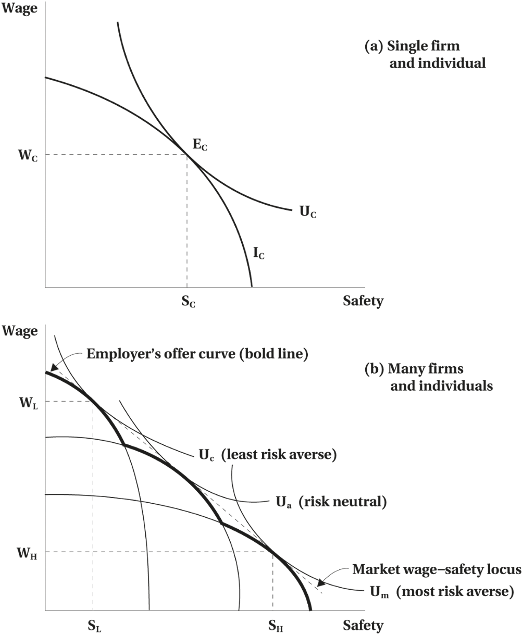
\includegraphics[width=0.79\linewidth]{ben54842_0803}
\end{frame}

\begin{frame}{Characteristics of the Wage -- Safety Locus}
\transfade
\begin{itemize}
  \item \textbf{Negative slope:} Lower safety must be compensated by higher wages.
  \item The shape depends on:
  \begin{itemize}
    \item worker preferences toward risk,
    \item firms' safety technologies.
  \end{itemize}
  \item The locus summarizes equilibrium outcomes across many firms and many workers.
\end{itemize}
\end{frame}



% ============================================================
\section{Effect of Safety Regulation}
% ============================================================

\begin{frame}{Regulation in Competitive Markets}
\transfade
\begin{itemize}
  \item In a frictionless competitive market, workers choose their preferred wage -- safety trade-off.
  \item If the market already reflects informed choices, a safety mandate may:
  \begin{itemize}
    \item lower wages,
    \item reduce firm profits,
    \item and potentially make some workers worse off.
  \end{itemize}
  \item But regulation may improve welfare if markets fail.
\end{itemize}
\end{frame}

\begin{frame}{Figure 8.4: Responses to a Safety Standard}
\centering
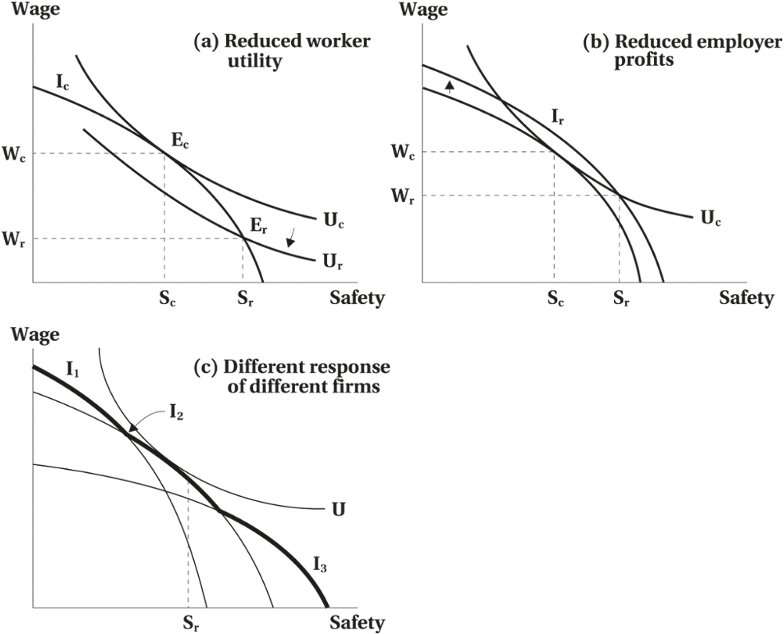
\includegraphics[width=0.59\linewidth]{ben54842_0804}
\end{frame}

\begin{frame}{Explaining Safety Standards}
\transfade
\begin{itemize}
  \item A mandated safety standard pushes firms toward safer jobs.
  \item This usually reduces the need for compensating wage premiums.
  \item Wages may fall because workers are receiving more safety instead of money.
  \item Whether regulation increases welfare depends on whether the original market outcome was efficient.
\end{itemize}
\end{frame}

\begin{frame}{Worked Example: Attracting Doctors to Rural Areas}
\transfade
\small
Two doctors can earn \$100{,}000 in a city.
\begin{itemize}
  \item Dr.\ Brown values city amenities at \$90{,}000:
  \[
  100{,}000 + 90{,}000 = 190{,}000
  \]
  so she needs about \$190{,}000 to be indifferent to moving rural.
  \item Dr.\ Lewis values city amenities at only \$40{,}000:
  \[
  100{,}000 + 40{,}000 = 140{,}000
  \]
  so she would move for a lower rural salary.
  \item \textbf{Implication:} Workers differ in the wage premium required to accept undesirable locations.
\end{itemize}
\end{frame}





\begin{frame}{Location Choice and Compensating Wage Differentials}
\transfade

\begin{center}
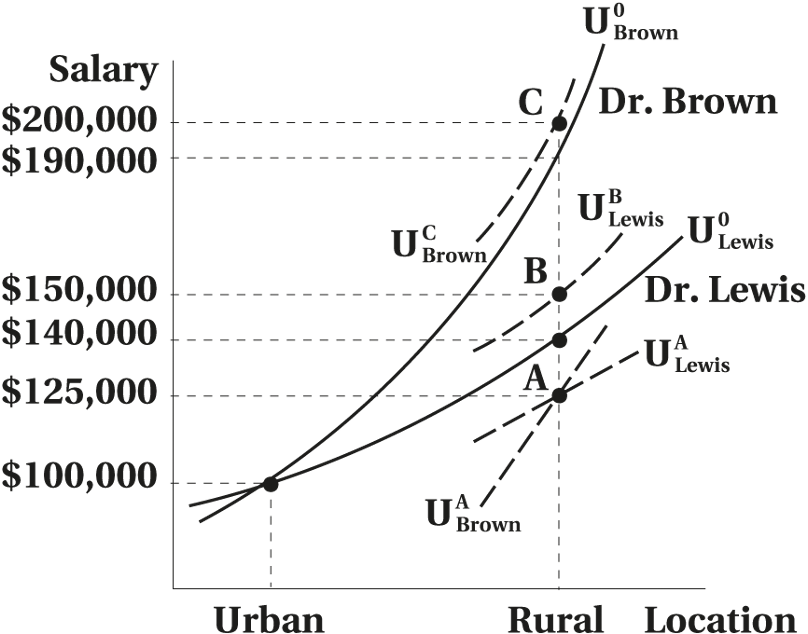
\includegraphics[width=0.6\linewidth]{ben54842_0801a}
\end{center}
\end{frame}

\begin{frame}{Location Choice and Compensating Wage Differentials}
\begin{itemize}

\item The vertical axis shows the worker's \textbf{salary}.

\item The horizontal axis shows the \textbf{job location}: Urban vs.\ Rural.

\item Both doctors earn about \textbf{\$100,000 in the urban location}.

\item Rural jobs must offer \textbf{higher wages} because many workers prefer urban amenities.

\item The curves labeled \(U\) represent \textbf{indifference curves}.

\item Each indifference curve shows combinations of \textbf{salary and location} that give the worker the \textbf{same level of utility}.

\end{itemize}

\end{frame}



\begin{frame}{Economic Interpretation of the Diagram}
\transfade

\begin{itemize}

\item Workers differ in how much they value \textbf{urban amenities} such as restaurants, schools, cultural life, and professional opportunities.

\item \textbf{Dr.\ Brown strongly prefers urban life}.  
She requires a much higher rural salary (around \$190,000) to be indifferent between urban and rural jobs.

\item \textbf{Dr.\ Lewis values urban amenities less}.  
She would be willing to move to a rural location for about \$140,000.

\item The difference between rural and urban wages represents a \textbf{compensating wage differential}.

\item Workers with stronger preferences for urban living require \textbf{larger wage premiums} to accept rural jobs.

\end{itemize}

\end{frame}



\begin{frame}{Example: Other Compensating Differentials}
\transfade
\begin{itemize}
  \item \textbf{Night shifts:} workers often receive a shift premium.
  \item \textbf{Remote locations:} jobs in northern or isolated areas often pay more.
  \item \textbf{Flexible work hours:} workers may accept lower wages in exchange for flexibility.
  \item \textbf{Health insurance or pensions:} these benefits often substitute for money wages.
\end{itemize}
\end{frame}

\begin{frame}{Imperfect Information}
\transfade
\begin{itemize}
  \item Workers may underestimate workplace risk.
  \item If workers misperceive risk, the market wage premium may be \textbf{too small}.
  \item In that case, safety regulation can improve:
  \begin{itemize}
    \item worker utility,
    \item market efficiency.
  \end{itemize}
  \item Better information can also move the market closer to the efficient outcome.
\end{itemize}
\end{frame}

\begin{frame}{Figure 8.5: Effect of Imperfect Information}
\centering
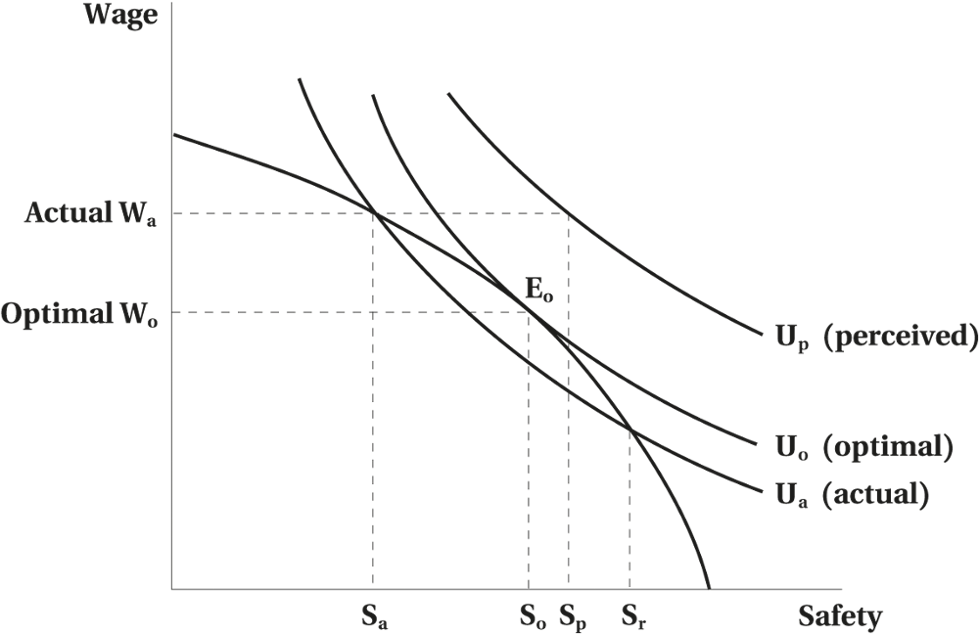
\includegraphics[width=0.69\linewidth]{ben54842_0805}
\end{frame}

\begin{frame}{Why Regulate?}
\transfade
\begin{itemize}
  \item \textbf{Information failures:} workers may not know the true risks.
  \item \textbf{Externalities:} workplace injuries may impose costs on families, insurers, or taxpayers.
  \item \textbf{Behavioural biases:} present bias, wishful thinking, and risk misperception may distort choices.
  \item \textbf{Imperfect competition:} firms may have monopsony power and under-compensate workers.
\end{itemize}
\end{frame}

% ============================================================
\section{Empirical Evidence on Compensating Wages}
% ============================================================

\begin{frame}{Methodological Challenges}
\transfade
\begin{itemize}
  \item \textbf{Simultaneous equation bias:} wages and job risk are jointly determined.
  \item \textbf{Errors in variables:} measured risk may be noisy or incomplete.
  \item \textbf{Omitted variables:} ability, preferences, and amenities may be unobserved.
  \item \textbf{Sample selection:} workers who choose risky jobs are not random.
\end{itemize}
\end{frame}

\begin{frame}{Wage -- Risk Trade-offs and Value of Life}
\transfade
\begin{itemize}
  \item Risk premia tend to rise with the severity of workplace hazards.
  \item Workers' compensation or insurance can reduce required wage premia.
  \item Economists estimate the \textbf{wage -- risk gradient} and use it to infer VSL.
  \item Example:
  \[
  VSL = \frac{\text{annual wage premium}}{\text{increase in fatality probability}}
  \]
\end{itemize}
\end{frame}



\begin{frame}{Desirable vs.\ Undesirable Job Characteristics}
\transfade
\begin{itemize}
  \item Empirical evidence often finds wage trade-offs for:
  \begin{itemize}
    \item health insurance,
    \item pensions,
    \item flexible schedules,
    \item workplace safety.
  \end{itemize}
  \item In some cases, wage offsets are incomplete because of market frictions or institutions.
\end{itemize}
\end{frame}

\begin{frame}{Employment Security}
\transfade
\begin{itemize}
  \item Jobs with higher layoff risk may require compensating wage premiums.
  \item However, public unemployment insurance can reduce the size of these premia.
  \item This makes empirical identification more difficult.
\end{itemize}
\end{frame}

\begin{frame}{Family-Friendly Work Practices}
\transfade
\begin{itemize}
  \item Family-friendly policies often behave like job amenities.
  \item Workers may accept lower wages for:
  \begin{itemize}
    \item flexible schedules,
    \item shorter commutes,
    \item parental leave,
    \item remote work.
  \end{itemize}
  \item Evidence is mixed for some policies, especially childcare support and work-from-home arrangements.
\end{itemize}
\end{frame}

\begin{frame}{Policy Implications}
\transfade
\begin{itemize}
  \item Uniform regulations may reduce welfare if workers differ greatly in preferences.
  \item Policies should account for:
  \begin{itemize}
    \item heterogeneity across workers,
    \item information problems,
    \item labour market institutions,
    \item existing insurance systems.
  \end{itemize}
  \item Compensating differentials help explain persistent wage patterns across jobs, industries, and regions.
\end{itemize}
\end{frame}

% ============================================================
\section{Chapter Summary}
% ============================================================

\begin{frame}{Summary}
\transfade
\begin{itemize}
  \item Compensating wage differentials price job attributes: workers trade wages for safety and amenities.
  \item Market equilibrium along a wage -- safety locus reflects both worker preferences and firm technologies.
  \item Regulation can improve outcomes under information failures, externalities, behavioural biases, or imperfect competition.
  \item Empirical estimation is difficult because wages and job characteristics are jointly determined.
  \item The theory helps explain why equally skilled workers can earn different wages across jobs.
\end{itemize}
\end{frame}

\begin{frame}
\centering
\Huge{\textbf{Thank You!}}
\end{frame}

\end{document}